\subsection{Strategies for Prediction}
\todo{present some of the strategies that we have towards prediction - maybe a summary of the above things?}
\subsubsection{Standard Inputs}

\subsubsection{Using Statistical Inputs}
\label{sec:usingStatisticalInput}
As described in the ANN section \todo{find method to point to page} in Figure~\ref{fig:overfitting} the Neural Network strives for a generalized function without overfitting so that it also applies for data outside of the trained set. In order to achieve such a function it is necessary to include enough input parameters to get a close enough fit. Every input parameter should narrow down the number of possible output values or else it makes no sense to include them. What can become problematic is when the input parameters simply result in too many output values, e.g. if similar wind speeds, air densities and temperatures would correspond to wind productions between 800-1300 \todo{concrete example from data set}. The generalization would move towards the majority of the wind productions in this interval but because the purpose of prediction is to come as close as possible to the ideal value this is not enough when the interval is too big. One way to solve this is to include a "snapshot" of the current situation as one or more input parameters so that it takes into account market trends at that time. As discussed in Historical Data~\ref{sec:historicalData} the market has certain trends \todo{ref} and if the prediction was to know the price from one hour ago and the current market trend in general it would have a better chance of guessing within the given interval. If putting this into context of the wind production interval 800-1300 --- if the last hour wind production was 1100 and the current trend is rising then the algorithm should with high probability not guess around 800 even if the majority of the wind productions is placed here. The concept is illustrated in Figure~\ref{fig:WP}\todo{make drawing}. By including the current trend as input the ANN could better approach the target to predict because it would result in a generalization of all trends in the dataset --- it would calculate how current trend in general influences the output over the entire dataset. If the majority of the rising trends in the dataset has a relatively small slope then the network would predict according to that. This will cause a problem when facing a steep slope because the ANN would not predict high enough. A solution could be to combine the statistical approach with curve analysis where the slope of the last prices and productions are taken into consideration as well. The slope says something about how much the curve is rising whereas the statistics will reflect the general trend over time. What makes it crucial is the wish to potentially predict the cases that are not general and irregular if it is possible.

Other problems arise together with the inclusion of tendency --- when have we moved enough in one direction? We need to rely on the other input parameters to pull us either up or down so that we can identify the next trend. This can possibly result in the prediction to significantly over-shoot or under-shoot its target. The statistical approach could potentially help out even more since it gives us the tool to calculate probability of the movement to come, e.g. what is the probability of the curve continuously moving up after 24. It will need to be tested thoroughly during our experiments. 

One thing to keep in mind here is that this is only a minority of the input parameters. Without these the Artificial Neural Network would have made one generalization and the addition would in theory only help the function to approach the target better when a lot of output possibilities exist. The result will be a new function where the immediate past is considered at every hour and the possibility of a improved generalization.

\begin{figure}[H]
\centering
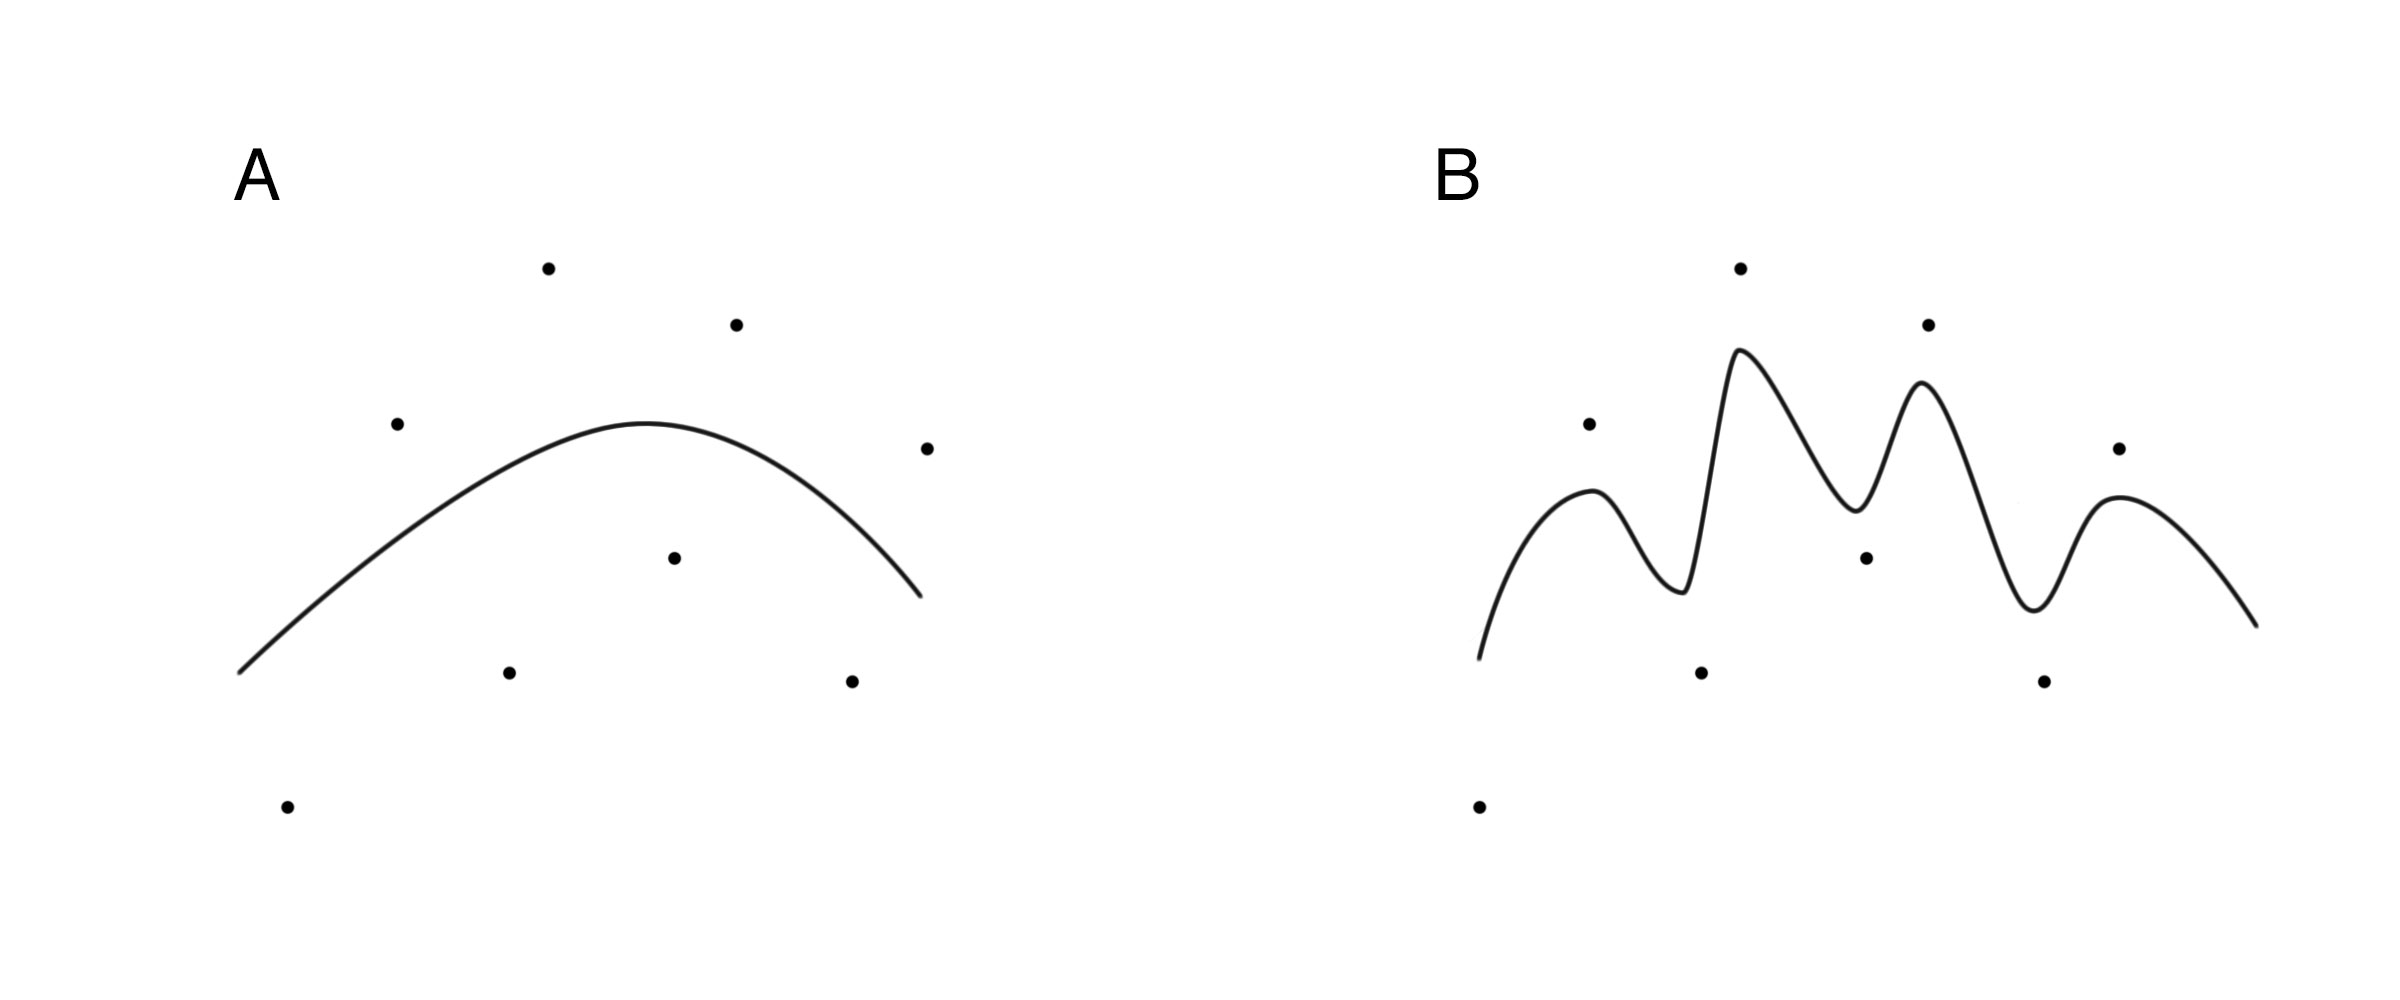
\includegraphics[width=0.99\linewidth,natwidth=898,natheight=587]{billeder/WP_000057.jpg}
\caption{A) Shows the generalized function. B) The approaching of output values}
\label{fig:WP}
\end{figure}

We will work with several statistical methods as input and with combinations of them all. 

\subsubsection{Statistical Input}
\todo{Talk about statistical input features like historical volatility (EWMA), skewness and basic calculation of line slope. Skewness is a more sophisticated way of calculating if the distribution is leaning to one sine of the mean - the simple line slope calculation is meant to calculate if we are on the way up or down}

EWMA should be used for time series that do not have a clear trend direction\cite[Chapter~7.3.2]{econometrics} which is exactly what we have. \todo{see page 588 in econometrics book}

The EWMA is a latent trend model where a latent variable is included to describe a discrete choice model. The latent variable is called the smoothing factor and if this factor is close to one then the last trend has a higher weight than the recent observation- in our case the observation would be either production or price and the smoothing factor is calculated based on the last calculated trend.

Choice of smoothing factor.

It has been used as an example for Industrial Production. 

TEGNING MULTIPE STEP

TALK ABOUT MULTIPLE-STEP-AHEAD FORECASTING --> see karlbranting
